% Canonical Phase C fixture: fictional technology/strategy deck.
% The pipeline manuscript uses the same trusted fragments below, proving that
% direct TeX and constrained Markdown authoring share the composition API.
\documentclass[theme=executive,publication-type=presentation]{reportkit-slides}

\setreportkitleftheader{NexaGrid / Strategy review}
\setreportkitfooter{NexaGrid Strategy Office -- fictional demonstration deck}
\setreportkitversion{v1.0}
\setreportkitsubject{NexaGrid decision velocity strategy}
\setreportkitkeywords{ReportKit, executive theme, strategy, fictional}
\title{Turn fragmented operational data into decision velocity}
\subtitle{A fictional technology strategy review}
\author{NexaGrid Strategy Office}
\date{20 September 2026}

\begin{document}

\begin{frame}[plain]
  \begin{titleslide}
  \end{titleslide}
\end{frame}

\begin{frame}
  \begin{evidenceslide}{Governance unlocks leverage before model expansion.}
    \begin{threepart}
  \threepartcolumn{Demand signal}{8 / 10 priority workflows show repeatable decision friction.}
  \threepartcolumn{Value pool}{\$18M of fictional annual leverage sits behind three workflow families.}
  \threepartcolumn{Binding constraint}{Data latency and ownership handoffs limit adoption more than model quality.}
\end{threepart}

  \end{evidenceslide}
\end{frame}

\begin{frame}
  \begin{architectureslide}[One semantic layer connects operating teams to reusable decisions.][Fictional NexaGrid target architecture.]
    \begin{diagram}[
  type=architecture,
  description={Three horizontal layers connect operating teams, decision services, and governed data contracts.}
]
  \begin{reportarchitecture}[width=14.2,annotation={One governed semantic layer connects operating teams to reusable decisions.},annotation-position=top]
    \layer{Decision layer}{Scenario cockpit, Alert routing}
    \layer{Intelligence layer}{Feature store, Policy engine}
    \layer{Foundation layer}{Contracts, Event lake}
  \end{reportarchitecture}
\end{diagram}

  \end{architectureslide}
\end{frame}

\begin{frame}
  \begin{fullvisual}[The operating loop turns signals into governed action.][Fictional NexaGrid decision workflow.]
    \begin{diagram}[
  type=flow,
  description={Four ordered steps move from detection through explanation and decision to learning.}
]
  \begin{reportflow}
    \step{detect}{Detect}
    \step{explain}{Explain}
    \step{decide}{Decide}
    \step{learn}{Learn}
    \flowedge{detect}{explain}
    \flowedge{explain}{decide}
    \flowedge{decide}{learn}
  \end{reportflow}
\end{diagram}

  \end{fullvisual}
\end{frame}

\begin{frame}
  \begin{visualtext}[left]{Prioritize the decision layer}{Scale the workflows that combine high value with a credible path to adoption.}
    \begin{diagram}[
  type=matrix,
  caption={Priorities by implementation effort and value at scale.},
  source={Fictional NexaGrid portfolio workshop.},
  description={A two by two priority matrix with four labelled workflow points.}
]
  \begin{reportmatrix}[width=6.3,height=4.6,xlabel={Implementation effort},ylabel={Value at scale},highlight=high/high]
    \quadrant{low}{high}{Prioritize}
    \quadrant{high}{high}{Sequence}
    \quadrant{low}{low}{Observe}
    \quadrant{high}{low}{Defer}
    \point{Exception routing}{.30}{.80}
    \point{Forecasting}{.52}{.68}
    \point[label-position=below]{Self-serve reporting}{.24}{.48}
    \point[label-position=below]{Automation}{.78}{.38}
  \end{reportmatrix}
\end{diagram}

  \end{visualtext}
\end{frame}

\begin{frame}
  \begin{chartslide}[right]{Adoption compounds before automation}{Removing rework from the operating model creates the capacity for better models and faster decisions.}
    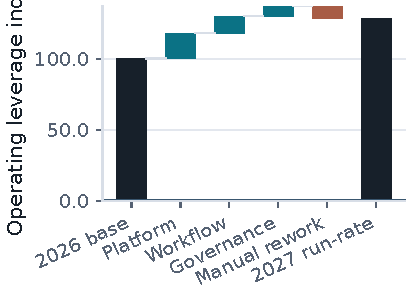
\includegraphics[width=\linewidth]{figures/adoption-bridge.pdf}

  \end{chartslide}
\end{frame}

\begin{frame}
  \begin{tableslide}[left]{Sequence the value pool}{Start with repeatable decisions, then extend the same contracts into adjacent teams.}
    {\small
\renewcommand{\arraystretch}{1.18}
\begin{tabular}{@{}>{\raggedright\arraybackslash}p{22mm}r >{\raggedright\arraybackslash}p{20mm}@{}}
\textbf{Initiative} & \textbf{Value} & \textbf{Readiness}\\[2pt]
Exception routing & \$7M & Pilot\\
Forecasting & \$6M & Design\\
Contract layer & \$5M & Scale\\
\end{tabular}
}

  \end{tableslide}
\end{frame}

\begin{frame}
  \begin{fullvisual}[Build gates and adoption milestones are managed as one plan.][Fictional NexaGrid 2027 delivery plan.]
    \begin{diagram}[
  type=timeline,
  description={Two-track timeline showing build gates above adoption milestones, with a decision gate before scale.}
]
  \begin{reporttimeline}[tracks={Build,Adoption},span=12]
    \event{Build}{.15}{Data contract}
    \event{Build}{.50}{Pilot}
    \event{Build}{.86}{Scale}
    \event{Adoption}{.28}{3 teams}
    \event{Adoption}{.68}{12 teams}
    \watermark[label-position=above]{Build}{.70}{decision gate}
  \end{reporttimeline}
\end{diagram}

  \end{fullvisual}
\end{frame}

\begin{frame}
  \begin{fullvisual}[The roadmap makes governance an enabling capability, not a final review step.][Fictional NexaGrid 2027 sequencing.]
    \begin{diagram}[
  type=roadmap,
  description={Three roadmap horizons cover contracts now, workflow pilots next, and scaled decision services later.}
]
  \begin{reportroadmap}[width=14.2]
    \horizon{Now}{Make trusted}{Contracts, Ownership}
    \horizon{Next}{Prove value}{Three pilots, Adoption loop}
    \horizon{Later}{Scale decisions}{Reusable services, Guardrails}
  \end{reportroadmap}
\end{diagram}

  \end{fullvisual}
\end{frame}

\begin{frame}[plain]
  \begin{messageslide}{Approve the governed decision layer as the 2027 platform priority.}
    \begin{itemize}
  \item Fund the governed contract layer and the first three workflow pilots.
  \item Sequence adoption milestones with build gates so value is visible early.
  \item Hold model expansion until ownership, latency, and feedback loops are measured.
\end{itemize}

\vspace{2mm}
\href{https://example.com/nexagrid-brief}{Open the fictional decision brief.}

  \end{messageslide}
\end{frame}

\end{document}
